\documentclass[a4paper,11pt,oneside]{article}  %bylo report
\usepackage[margin=0.75in]{geometry}
\usepackage[utf8]{inputenc} %ISO-8859-2 
\usepackage[polish]{babel} 
%\usepackage{times} 
\usepackage[T1]{fontenc} 
\usepackage[MeX]{polski} 
\usepackage[pdftex]{graphicx} 
\usepackage{pdfpages} 
\usepackage{fancyhdr} %numery stron po zewnętrznej 
\usepackage{wrapfig}
\usepackage[colorlinks=true,bookmarksopen,plainpages=false,urlcolor=blue,citecolor=black,filecolor=black,linkcolor=black,,unicode]{hyperref} 
\usepackage{titlesec} 
\usepackage{booktabs}
\usepackage{attachfile}
\usepackage{appendix}
\usepackage{listings}
\usepackage{tikz}
\usetikzlibrary{shapes,arrows,fit} %use shapes library if you need ellipse
\title{Moduł akwizycji czujnika UFXC\\ Propozycja systemu wyzwalania \\[10pt] \large{Creotech Instruments S.A.} \\ \large{Akademia Górniczo Hutnicza w Krakowie}}
\author{Piotr Zdunek}

\usepackage{newunicodechar}
\newunicodechar{fi}{fi}
\usepackage{courier}
\usepackage{listings}
\usepackage{float}
\pdfminorversion=5 
\pdfcompresslevel=9
\pdfobjcompresslevel=2
\usepackage{multirow}
\usepackage{url}
\usepackage{graphics}
\usepackage[section]{placeins}


\begin{document}
%\maketitle 
%
%\begin{table}[h]
%  \centering
%  \begin{tabular}{| c | c | c |}
%    \cline{1-3}  \textbf{Skład zespołu} & \textbf{Przedmiot} & \textbf{Data} \\
%   \hline
% 	Piotr Zdunek 	& \multirow{2}{*}{ Metody i~systemy pomiarowe wielkiej częstotliwości} & \multirow{2}{*}{07.04.2014} \\[5pt]
% 	Paweł Gontarek & & \\
%   \hline
%   \textbf{Prowadzący} 		& \textbf{Tytuł ćwiczenia}	&	\textbf{Numer stanowiska} \\
%   \hline
%   dr~inż. Wojciech Wiatr	&	Pomiar parametrów materiałowych metodą rezonansową	&	2			\\
%   \hline
%  \end{tabular}
%    \label{tab:tytulowa}
%\end{table}





\maketitle


\lstdefinestyle{custom}{
  belowcaptionskip=1\baselineskip,
  breaklines=true,
  frame=L,
  xleftmargin=\parindent,
  language=Matlab,
  showstringspaces=false,
  basicstyle=\footnotesize\ttfamily,
  keywordstyle=\bfseries\color{green!40!black},
  commentstyle=\itshape\color{purple!40!black},
  identifierstyle=\color{blue},
  stringstyle=\color{orange},
}

\lstset{escapechar=@,style=custom}

%\tableofcontents
%\newpage	
\section{Wstęp} 
Dokument opisuje propozycję realizacji systemu wyzwalania pomiaru z czujnika UFXC w systemie akwizycji i sterowania. 

\section{Założenia}

\begin{itemize}
\item możliwość wyzwalania (akwizycji ramki) sygnałem zewnętrznym albo wewnętrznym
\item wyzwalanie wewnętrzne może być uruchamiane za pomocą programu sterującego bądź poprzez sygnał zewnętrzny
\item zapewnienie synchronizacji modułów
\end{itemize}




\section{Propozycja realizacji}

System wyzwalania rozpatrujemy w scenariuszu gdy kilka modułów pracuje wspólnie. Poza możliwością komunikacji poprzez sieć Ethernet moduły połączone są ze sobą 8 liniami LVDS doprowadzonymi do modułów za pomocą taśmy wpinanej do złącz IDC. Tymi liniami będą przesłane sygnały zegarowe i wyzwalania. W docelowej obudowie na cały system taśma zostanie wyprowadzona na zewnątrz z wykorzystaniem przejściówki na złącza LEMO bądź SMA (do ustalenia). 

\paragraph{Synchronizacja}
Sygnał zegarowy służy do synchronizacji modułów między sobą. Może zostać wygenerowany przez jeden z modułów albo doprowadzony z zewnątrz. 

\paragraph{Wyzwalanie}

Wyzwalanie pomiaru będzie wykonywane za pomocą wewnętrznego bądź zewnętrznego sygnału. Wewnętrzne wyzwalanie będzie sterowane ze pomocą protokołu TCP albo za pomocą zewnętrznego sygnału wyzwalającego. Akwizycja wewnętrzna będzie wykonana określoną ilość razy ze stałym odstępem czasowym (Tacq) (zgodnie z \cite{SPEC}). 

Natomiast zewnętrzne wyzwalanie będzie sterowane tylko za pomocą zewnętrznego sygnału doprowadzonego na wejście systemu sterowania. Akwizycja pojedyńczej ramki będzie wykonana wzlgędem sygnału zegara synchronizacyjnego. 

\paragraph{Przykład}
Chcemy zebrać jedną ramkę z baterii czujników. Doprowadzamy na wejście systemu sygnał zegarowy o częstotliwości 100 MHz. Natomiast na wejście wyzwalania podajemy pojedynczy impuls prostokątny, o okresie większym niż połowa okresu sygnału zegara, ale mniejszym od całego okresu - tak aby zebrać pojedynczą ramkę. Akwizycja jest wyzwalana na narastające zbocze zegara synchronizacyjnego (do ustalenia).

\begin{figure}[!h]
	\centering
	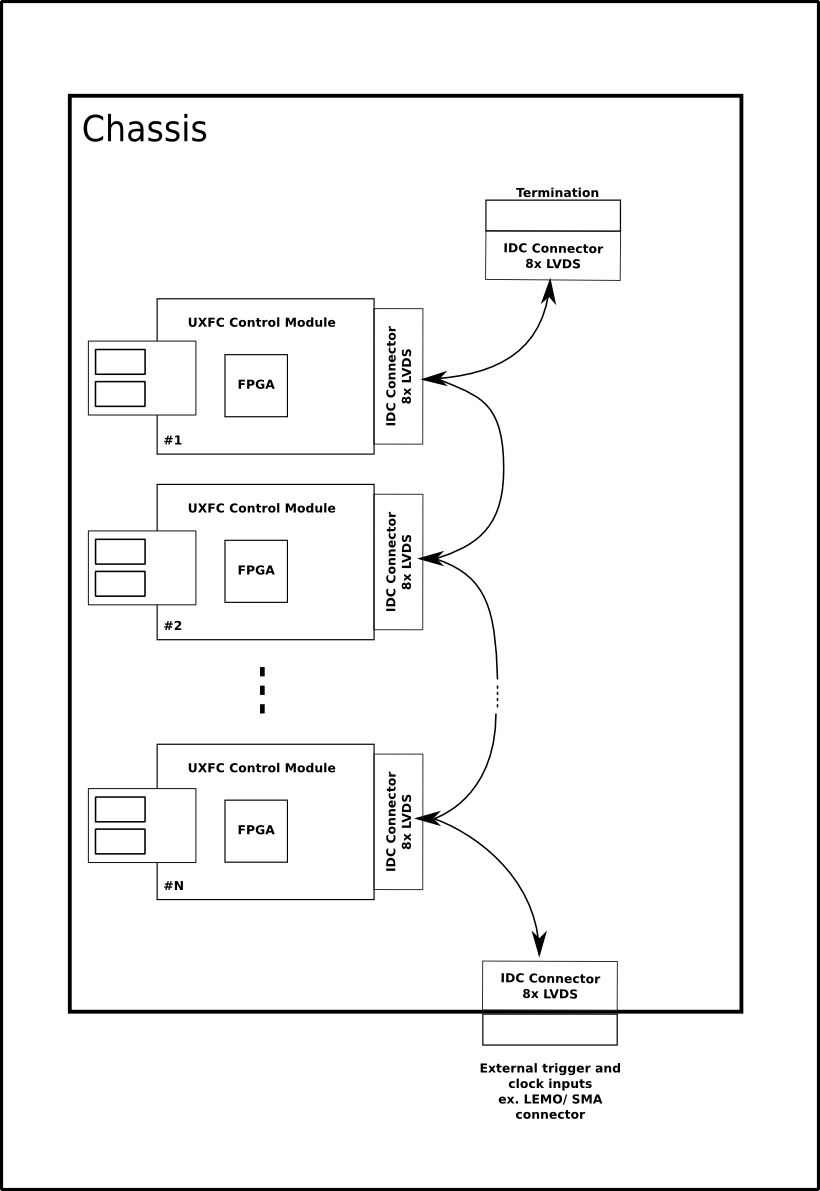
\includegraphics[width=16cm]{trigger_sync.png}
	\caption{Schemat blokowy systemu wyzwalania}
	\label{fig:SYS}
\end{figure}


\begin{thebibliography}{9}
\bibitem{SPEC} Specyfikacja wymagań modułu odczytowgeo układu UFXC - Firmware

	


\end{thebibliography}
\end{document}
